\documentclass[crop,tikz]{standalone}

\usepackage{pgfplots}
\colorlet{green}{black!40!green}

\tikzset{>=latex}

\pgfplotsset{
  every non boxed x axis/.append style={
    axis line style={-latex}
  },
  every non boxed y axis/.append style={
    axis line style={-latex}
  },
  inverted/.style = {
    every axis legend/.append style={
      draw=white,
      fill=black,
      text=white
    }
  }
}

\begin{document}
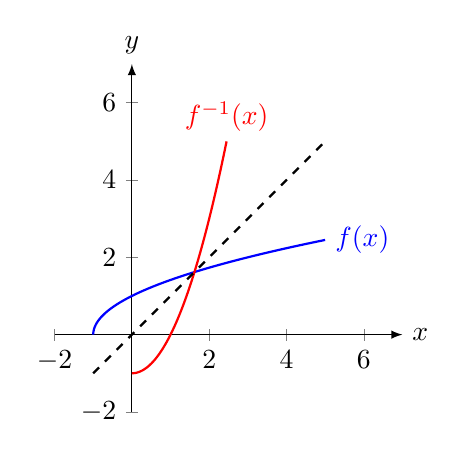
\begin{tikzpicture}
\begin{axis}[
  width=6cm,
  height=6cm,
  xlabel={$x$},          % default put x on x-axis
  ylabel={$y$},          % default put y on y-axis
  xmin = -2, xmax = 7,
  ymin = -2, ymax = 7,
  axis y line=middle,
  axis x line=middle,
  xlabel style={at=(current axis.right of origin), anchor=west},
  ylabel style={at=(current axis.above origin), anchor=south},
  samples=100,
  smooth,
  ]
  \addplot[blue, domain=0:{sqrt(6)}, thick] ({x^2-1},x) node[right] {$f(x)$};
  \addplot[red, domain=0:{sqrt(6)}, thick] {x^2-1} node[above] {$f^{-1}(x)$};
  \addplot[dashed, domain=-1:5, thick] {x};
\end{axis}
\end{tikzpicture}
\end{document}
